% Created 2021-09-27 Mon 12:02
% Intended LaTeX compiler: xelatex
\documentclass[letterpaper]{article}
\usepackage{graphicx}
\usepackage{grffile}
\usepackage{longtable}
\usepackage{wrapfig}
\usepackage{rotating}
\usepackage[normalem]{ulem}
\usepackage{amsmath}
\usepackage{textcomp}
\usepackage{amssymb}
\usepackage{capt-of}
\usepackage{hyperref}
\setlength{\parindent}{0pt}
\usepackage[margin=1in]{geometry}
\usepackage{fontspec}
\usepackage{svg}
\usepackage{cancel}
\usepackage{indentfirst}
\setmainfont[ItalicFont = LiberationSans-Italic, BoldFont = LiberationSans-Bold, BoldItalicFont = LiberationSans-BoldItalic]{LiberationSans}
\newfontfamily\NHLight[ItalicFont = LiberationSansNarrow-Italic, BoldFont       = LiberationSansNarrow-Bold, BoldItalicFont = LiberationSansNarrow-BoldItalic]{LiberationSansNarrow}
\newcommand\textrmlf[1]{{\NHLight#1}}
\newcommand\textitlf[1]{{\NHLight\itshape#1}}
\let\textbflf\textrm
\newcommand\textulf[1]{{\NHLight\bfseries#1}}
\newcommand\textuitlf[1]{{\NHLight\bfseries\itshape#1}}
\usepackage{fancyhdr}
\pagestyle{fancy}
\usepackage{titlesec}
\usepackage{titling}
\makeatletter
\lhead{\textbf{\@title}}
\makeatother
\rhead{\textrmlf{Compiled} \today}
\lfoot{\theauthor\ \textbullet \ \textbf{2021-2022}}
\cfoot{}
\rfoot{\textrmlf{Page} \thepage}
\renewcommand{\tableofcontents}{}
\titleformat{\section} {\Large} {\textrmlf{\thesection} {|}} {0.3em} {\textbf}
\titleformat{\subsection} {\large} {\textrmlf{\thesubsection} {|}} {0.2em} {\textbf}
\titleformat{\subsubsection} {\large} {\textrmlf{\thesubsubsection} {|}} {0.1em} {\textbf}
\setlength{\parskip}{0.45em}
\renewcommand\maketitle{}
\author{Houjun Liu, Exr0n}
\date{\today}
\title{Capacitors}
\hypersetup{
 pdfauthor={Houjun Liu, Exr0n},
 pdftitle={Capacitors},
 pdfkeywords={},
 pdfsubject={},
 pdfcreator={Emacs 28.0.50 (Org mode 9.4.4)}, 
 pdflang={English}}
\begin{document}

\tableofcontents

\#ref

\section{Capacitors vs. Batteries}
\label{sec:orgf70b190}
\textbf{Batteries} => Converting \(PE_{chem}\) => Eletrical energy

\textbf{Capacitors} => Converting \(PE_{elec}\) => Eletrical energy

When you are discharging a battery, they remain at constant voltage
until they are used up, at which point the voltage drop like a plate.

When you are discharging a capacitor, there is a linear fall in voltage
that is constant.

Charge remaining: capacitance times voltage

\section{Energy on a Capacitor}
\label{sec:org2a89280}
A little bit \#disorganized

Energy stored on a capacitor: \(E=\frac{V_c * Q}{2}\).

Charge on a capacitor: \(Q = C \times V_c\)

Farads: \(F = \frac{C}{V}\)

So, putting this together, the energy stored on a capacitor would be\ldots{}

\definition[as $Q=C \times V_c$]{Energy stored in a capacitor}\{\(E=\frac{V \times Q}{2} = \frac{CV^2}{2}\)\}
\(Q_{cap} \propto V\). In fact \(Q_{cap} = C \times V_c\).

\section{Capacitors interacting with Resistance}
\label{sec:org0302068}
As you increase the
\href{KBhPHYS201ResistanceConductivity.org}{KBhPHYS201ResistanceConductivity},
the a capacitor of the same capacitance would charge slower. (\emph{"Less
charge flows in"})

As you fix the Resistance, the capacitor of a higher capacitance would
charge slower. (\emph{"Need more change to fill"})

\begin{figure}[htbp]
\centering
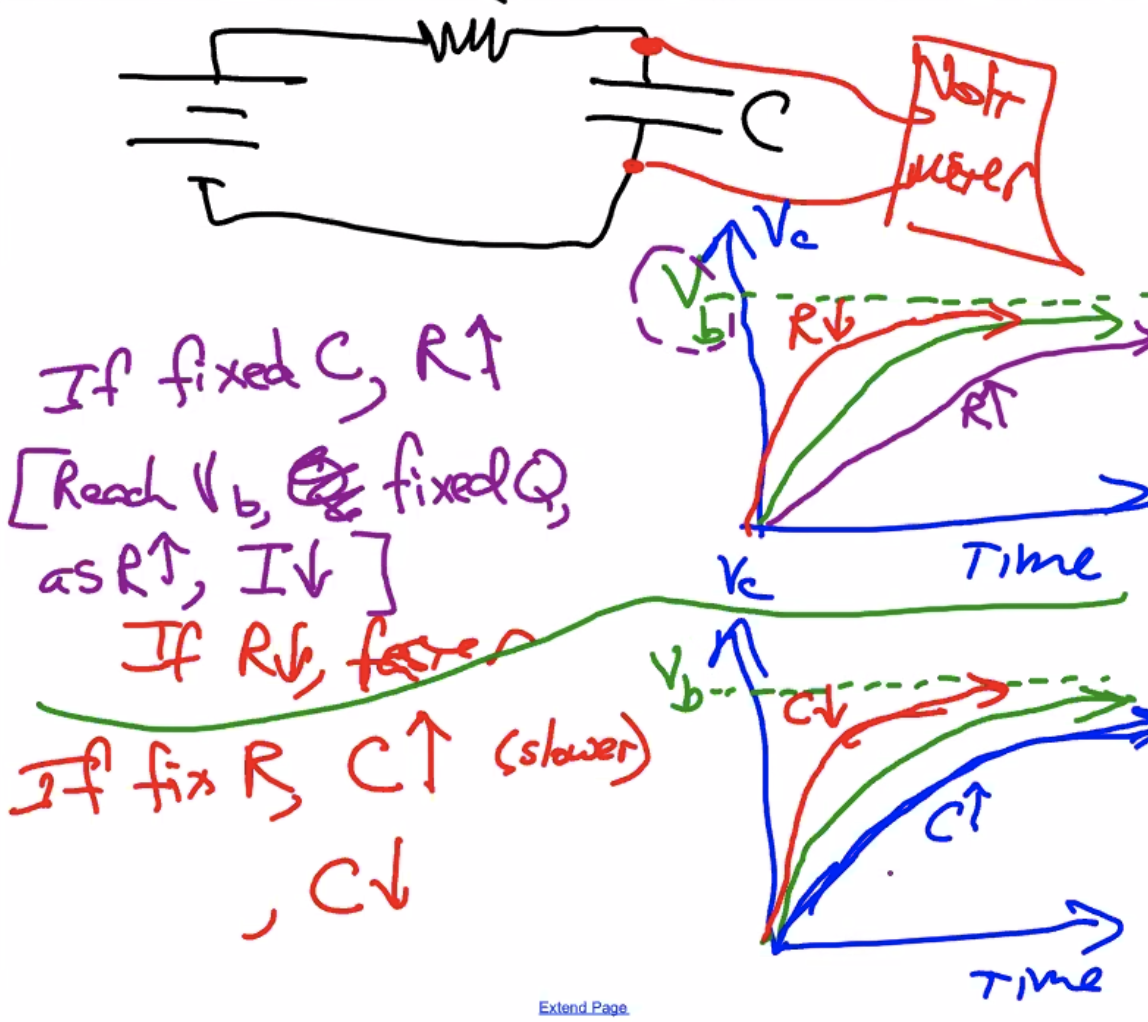
\includegraphics[width=.9\linewidth]{Screen Shot 2020-09-30 at 10.42.44 AM.png}
\caption{Screen Shot 2020-09-30 at 10.42.44 AM.png}
\end{figure}

\emph{Charging time} is in fairly good agreement with \emph{resistance times
capacitance}.

So\ldots{} \#disorganized

Experimentally, "Charging time", \(\tau\) \(\approx R \times C\).

Let's check the units!

\begin{itemize}
\item \(V = IR\)

\item \(R = \frac{V}{I}\)

\item So \(R = \omega = \frac{V * s}{Q}\)

\item \(Q = CV\)

\item So \(\frac{Q}{V} = C\)
\end{itemize}

Hence,
\(R \times C = \frac{\cancel{V} \times s}{\cancel{Q}} = \cancel{\frac{Q}{V}}\),
indeed, has a unit Seconds!

\section{Equations modeling charging a capacitor}
\label{sec:orgd0b89c4}
\definition[where $R$ is the resistance, $C$ is the capacitance]{Time Constant Tau}{$RC = \tau$ — time constant to be able to change the capacitor to a useful voltage; aka how much does the capacitor need to noticeably charge/discharge.}
Now that we have this value, we could also represent the full charge
process using the equations as follows:

\definition[where $V_b$ is the battery voltage, $t$ is time elapsed, $R$ is resistance, and $C$ is the capacitance]{Current in circuit as you charge a capacitor}\{\(I(t) = \frac{V_b}{R} \times e^{\frac{-t}{RC}}\)\}
As you start to charge a capacitor, the current starts at
\(\frac{V_b}{R}\) --- current just without the resistor. Then, it will
slowly drop down to 0.

\definition[where $V_b$ is the battery voltage, $t$ is time elapsed, $R$ is resistance, and $C$ is the capacitance]{Voltage before and after a capacitor as you charge a capacitor}\{\(V(t) = V_b \times (1 - e^{\frac{-t}{RC}})\)\}
\#disorganized

\section{Capacitors in series and parallel}
\label{sec:org025b2db}
Helpful to see:
\href{KBhPHYS201CombiningResistors.org}{KBhPHYS201CombiningResistors}

\subsection{Capacitors in Parallel}
\label{sec:org57ac3d3}
\begin{figure}[htbp]
\centering
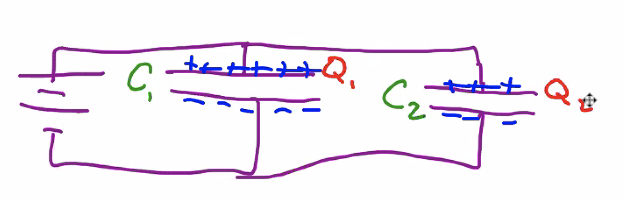
\includegraphics[width=.9\linewidth]{Screen Shot 2020-10-07 at 10.20.06 AM.png}
\caption{Screen Shot 2020-10-07 at 10.20.06 AM.png}
\end{figure}

\(Q_{tot} = Q_1 + Q_2\).

And, because of the fact that \(C = \frac{Q}{V}\),
\(V\times C_{eq} = V \times C_1 + V \times C_2\)

Dividing \(V\) out of the previous equations \(C_{eq} = C_1 + C_2\).

\textbf{Capacitors in parallel act like resistors in series.}

\subsection{Capacitors in Series}
\label{sec:orgb0268da}
\begin{figure}[htbp]
\centering
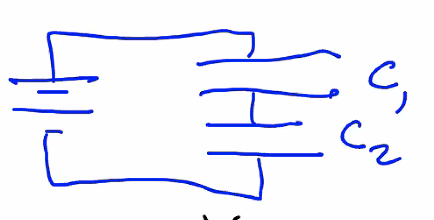
\includegraphics[width=.9\linewidth]{Screen Shot 2020-10-07 at 10.23.08 AM.png}
\caption{Screen Shot 2020-10-07 at 10.23.08 AM.png}
\end{figure}

Because of the fact that the middle wire does not carry any changes, it
is "neutral" and simply polarized --- making \(Q_1\) equaling \(Q_2.\)

Why is this? If the middle bit is neutral, the \(Q^+\) on one end would
equal to the \(Q^-\) on the other. Correspondingly, the other side of
the plates of the capacitor would have the opposite of the same values
\(Q^-\) and \(Q^+\) on the neutral middle plate.

By the transitive property, \(Q_1 = Q_2\).

Because \(V_1 + V_2 = V_b\) --- see
\href{KBhPHYS201CombiningResistors.org}{KBhPHYS201CombiningResistors}
\& \(C = \frac{Q}{V}\) ,
\(\frac{Q_1}{V} + \frac{Q_2}{V} = \frac{Q_{tot}}{V}\).

Given \(Q_1 = Q_2\).

So

\subsection{Construction of Capacitors}
\label{sec:org50528ea}
A diagram of the plates inside a polar capacitor before being rolled up.

\begin{center}
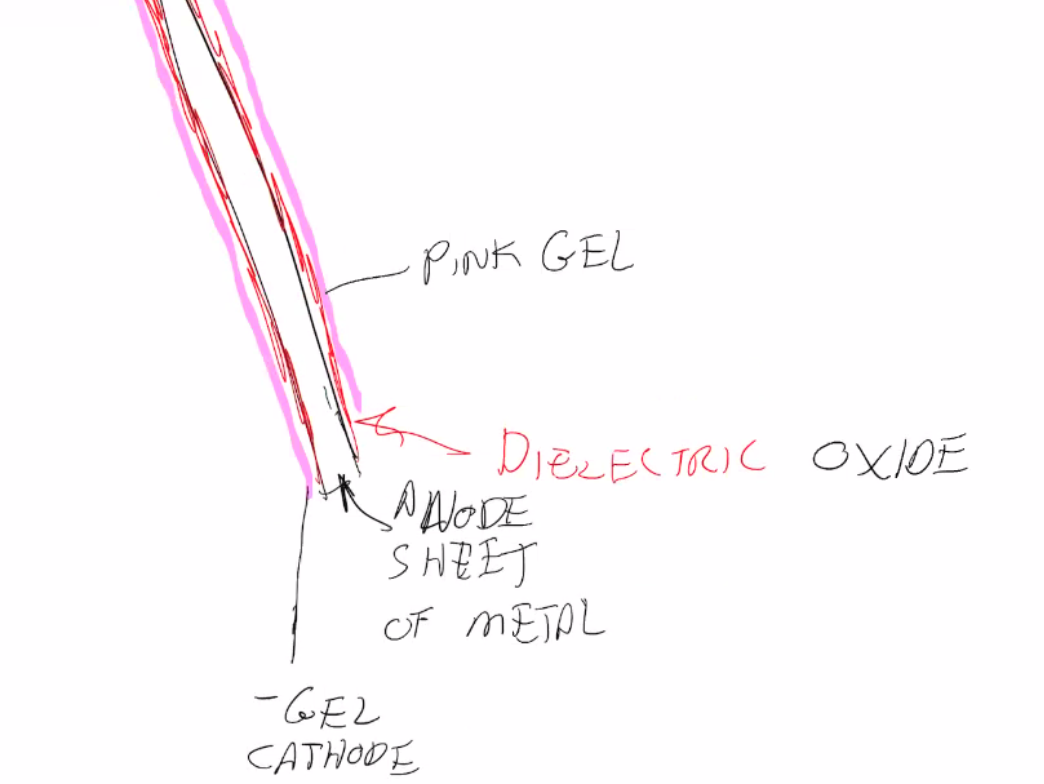
\includegraphics[width=.9\linewidth]{./Pastedimage20201007131933.png}
\end{center}
\end{document}
